\documentclass[12pt,a4paper]{article}
\usepackage{tikz}
\usetikzlibrary{arrows,snakes,backgrounds,patterns,shapes.geometric,calc}

\begin{document}
	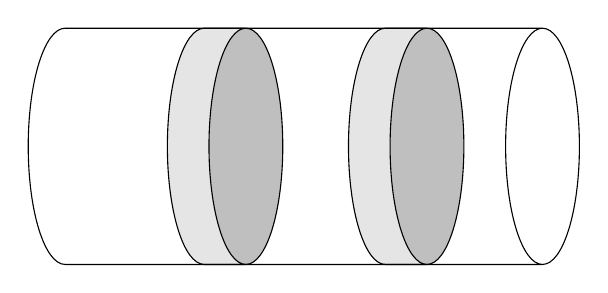
\begin{tikzpicture}[scale=1]
	\node [draw, cylinder, cylinder uses custom fill, cylinder body fill=gray!20, 
	cylinder end fill=gray!50, shape aspect=4, rotate=0, minimum width=3cm] (c1) at 
	(1.3,0){};
	\node [draw, cylinder, cylinder uses custom fill, cylinder body fill=gray!20, 
	cylinder end fill=gray!50, shape aspect=4, rotate=0, minimum width=3cm] (c2) at 
	(-1,0){};
	
	\node [draw, cylinder, cylinder body fill=gray!20, 
	cylinder end fill=gray!50, shape aspect=4, rotate=0, minimum height=7cm, minimum 
	width=3cm] (c) {};
	
	\coordinate(htop) at ($(c.before top)!-1*.1!(c.after top)$);
	\coordinate(hbot) at ($(c.after bottom)!-1*.1!(c.before bottom)$);
	\coordinate(hlabel) at ($(htop)!.5!(hbot)+(c.north)!.9!(c.center)$);
	
	%\draw[|-|] (hbot)--(htop);
	%\path (hlabel) node[left] {$h$}; %Modify height label here
	
	\coordinate (center) at ($(c.before top)!0.5!(c.after top)$);
	
	\coordinate (rlabel) at ($(center) !0.5!(c.after top)$);
	\coordinate (rtop) at ($(center)!-1*.1!(c.after top)$);
	\end{tikzpicture}
\end{document}